\documentclass{ximera}
\graphicspath{  %% When looking for images,
{./}            %% look here first,
{./pictures/}   %% then look for a pictures folder,
{../pictures/}  %% which may be a directory up.
{../../pictures/}  %% which may be a directory up.
{../../../pictures/}  %% which may be a directory up.
{../../../../pictures/}  %% which may be a directory up.
}

\usepackage{listings}
%\usepackage{circuitikz}
\usepackage{xcolor}
\usepackage{amsmath,amsthm}
\usepackage{subcaption}
\usepackage{graphicx}
\usepackage{tikz}
%\usepackage{tikz-3dplot}
\usepackage{amsfonts}
%\usepackage{mdframed} % For framing content
%\usepackage{tikz-cd}

  \renewcommand{\vector}[1]{\left\langle #1\right\rangle}
  \newcommand{\arrowvec}[1]{{\overset{\rightharpoonup}{#1}}}
  \newcommand{\ro}{\texttt{R}}%% row operation
  \newcommand{\dotp}{\bullet}%% dot product
  \renewcommand{\l}{\ell}
  \let\defaultAnswerFormat\answerFormatBoxed
  \usetikzlibrary{calc,bending}
  \tikzset{>=stealth}
  




%make a maroon color
\definecolor{maroon}{RGB}{128,0,0}
%make a dark blue color
\definecolor{darkblue}{RGB}{0,0,139}
%define the color fourier0 to be the maroon color
\definecolor{fourier0}{RGB}{128,0,0}
%define the color fourier1 to be the dark blue color
\definecolor{fourier1}{RGB}{0,0,139}
%define the color fourier 1t to be the light blue color
\definecolor{fourier1t}{RGB}{173,216,230}
%define the color fourier2 to be the dark green color
\definecolor{fourier2}{RGB}{0,100,0}
%define teh color fourier2t to be the light green color
\definecolor{fourier2t}{RGB}{144,238,144}
%define the color fourier3 to be the dark purple color
\definecolor{fourier3}{RGB}{128,0,128}
%define the color fourier3t to be the light purple color
\definecolor{fourier3t}{RGB}{221,160,221}
%define the color fourier0t to be the red color
\definecolor{fourier0t}{RGB}{255,0,0}
%define the color fourier4 to be the orange color
\definecolor{fourier4}{RGB}{255,165,0}
%define the color fourier4t to be the darker orange color
\definecolor{fourier4t}{RGB}{255,215,0}
%define the color fourier5 to be the yellow color
\definecolor{fourier5}{RGB}{255,255,0}
%define the color fourier5t to be the darker yellow color
\definecolor{fourier5t}{RGB}{255,255,100}
%define the color fourier6 to be the green color
\definecolor{fourier6}{RGB}{0,128,0}
%define the color fourier6t to be the darker green color
\definecolor{fourier6t}{RGB}{0,255,0}

%New commands for this doc for errors in copying
\newcommand{\eigenvar}{\lambda}
%\newcommand{\vect}[1]{\mathbf{#1}}
\renewcommand{\th}{^{\text{th}}}
\newcommand{\st}{^{\text{st}}}
\newcommand{\nd}{^{\text{nd}}}
\newcommand{\rd}{^{\text{rd}}}
\newcommand{\paren}[1]{\left(#1\right)}
\newcommand{\abs}[1]{\left|#1\right|}
\newcommand{\R}{\mathbb{R}}
\newcommand{\C}{\mathbb{C}}
\newcommand{\Hilb}{\mathbb{H}}
\newcommand{\qq}[1]{\text{#1}}
\newcommand{\Z}{\mathbb{Z}}
\newcommand{\N}{\mathbb{N}}
\newcommand{\q}[1]{\text{``#1''}}
%\newcommand{\mat}[1]{\begin{bmatrix}#1\end{bmatrix}}
\newcommand{\rref}{\text{reduced row echelon form}}
\newcommand{\ef}{\text{echelon form}}
\newcommand{\ohm}{\Omega}
\newcommand{\volt}{\text{V}}
\newcommand{\amp}{\text{A}}
\newcommand{\Seq}{\textbf{Seq}}
\newcommand{\Poly}{\textbf{P}}
\renewcommand{\quad}{\text{    }}
\newcommand{\roweq}{\simeq}
\newcommand{\rowop}{\simeq}
\newcommand{\rowswap}{\leftrightarrow}
\newcommand{\Mat}{\textbf{M}}
\newcommand{\Func}{\textbf{Func}}
\newcommand{\Hw}{\textbf{Hamming weight}}
\newcommand{\Hd}{\textbf{Hamming distance}}
\newcommand{\rank}{\text{rank}}
\newcommand{\longvect}[1]{\overrightarrow{#1}}
% Define the circled command
\newcommand{\circled}[1]{%
  \tikz[baseline=(char.base)]{
    \node[shape=circle,draw,inner sep=2pt,red,fill=red!20,text=black] (char) {#1};}%
}

% Define custom command \strikeh that just puts red text on the 2nd argument
\newcommand{\strikeh}[2]{\textcolor{red}{#2}}

% Define custom command \strikev that just puts red text on the 2nd argument
\newcommand{\strikev}[2]{\textcolor{red}{#2}}

%more new commands for this doc for errors in copying
\newcommand{\SI}{\text{SI}}
\newcommand{\kg}{\text{kg}}
\newcommand{\m}{\text{m}}
\newcommand{\s}{\text{s}}
\newcommand{\norm}[1]{\left\|#1\right\|}
\newcommand{\col}{\text{col}}
\newcommand{\sspan}{\text{span}}
\newcommand{\proj}{\text{proj}}
\newcommand{\set}[1]{\left\{#1\right\}}
\newcommand{\degC}{^\circ\text{C}}
\newcommand{\centroid}[1]{\overline{#1}}
\newcommand{\dotprod}{\boldsymbol{\cdot}}
%\newcommand{\coord}[1]{\begin{bmatrix}#1\end{bmatrix}}
\newcommand{\iprod}[1]{\langle #1 \rangle}
\newcommand{\adjoint}{^{*}}
\newcommand{\conjugate}[1]{\overline{#1}}
\newcommand{\eigenvarA}{\lambda}
\newcommand{\eigenvarB}{\mu}
\newcommand{\orth}{\perp}
\newcommand{\bigbracket}[1]{\left[#1\right]}
\newcommand{\textiff}{\text{ if and only if }}
\newcommand{\adj}{\text{adj}}
\newcommand{\ijth}{\emph{ij}^\text{th}}
\newcommand{\minor}[2]{M_{#2}}
\newcommand{\cofactor}{\text{C}}
\newcommand{\shift}{\textbf{shift}}
\newcommand{\startmat}[1]{
  \left[\begin{array}{#1}
}
\newcommand{\stopmat}{\end{array}\right]}
%a command to give a name to explorations and hints and theorems
\newcommand{\name}[1]{\begin{centering}\textbf{#1}\end{centering}}
\newcommand{\vect}[1]{\vec{#1}}
\newcommand{\dfn}[1]{\textbf{#1}}
\newcommand{\transpose}{\mathsf{T}}
\newcommand{\mtlb}[2][black]{\texttt{\textcolor{#1}{#2}}}
\newcommand{\RR}{\mathbb{R}} % Real numbers
\newcommand{\id}{\text{id}}
\newcommand{\coord}[1]{\langle#1\rangle}
\newcommand{\RREF}{\text{RREF}}
\newcommand{\Null}{\text{Null}}
\newcommand{\Nullity}{\text{Nullity}}
\newcommand{\Rank}{\text{Rank}}
\newcommand{\Col}{\text{Col}}
\newcommand{\Ef}{\text{EF}}
\newcommand{\boxprod}[3]{\abs{(#1\times#2)\cdot#3}}

\author{Zack Reed}
%borrowed from Ana Davis
\title{Orthogonal Projections}
\begin{document}
\begin{abstract}


\end{abstract}
\maketitle


    \section*{Orthogonal Projections}

    One of the most useful concepts in linear algebra that has numerous applications in further mathematics course and in varoius applications is the idea of \emph{orthogonal} projection. This builds on the more familiar idea of \emph{perpendicular} lines and \emph{right angles} from geometry in prior courses, but in a meaningful way that extends to higher dimensions. 

    \subsection*{Planes, Lines, and Angles}

    In prior sections, we considered lines in $\RR^n$ to be the span of a single vector, and planes in $\RR^n$ to be the span of two (linearly independent) vectors. 

    \begin{center}
      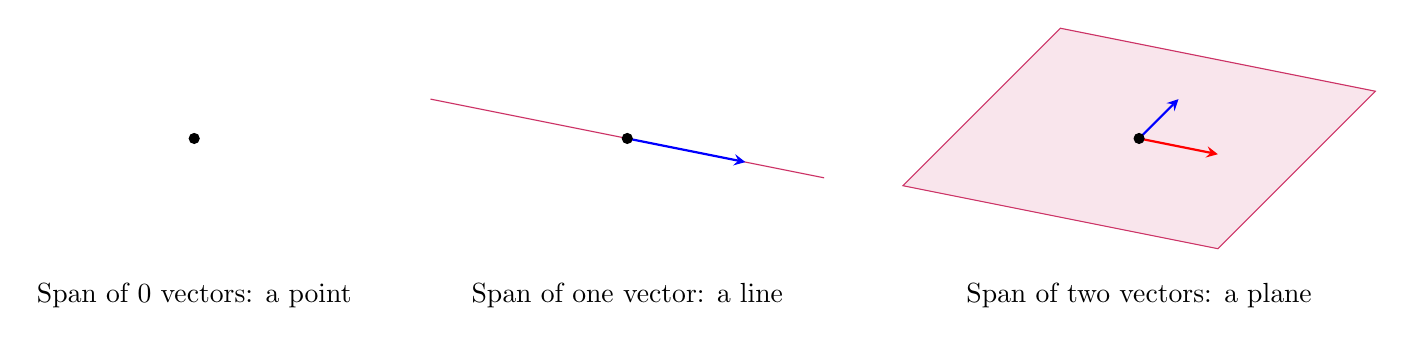
\begin{tikzpicture}
        \begin{scope}[xshift=-6cm]
          \draw[fill](0,0) circle [radius=1.8pt];
          \path(0,-2) node {Span of 0 vectors: a point};
        \end{scope}
        \begin{scope}[xshift=-0.5cm]
          \begin{scope}[x={(1cm,-0.2cm)},y={(0.5cm,0.5cm)}]
            \draw[purple!80](-2.5,0) -- (2.5,0);
            \draw[->, thick, blue](0,0) -- +(1.5,0);
            \draw[fill](0,0) circle [radius=1.8pt];
          \end{scope}
          \path(0,-2) node {Span of one vector: a line};
        \end{scope}
        \begin{scope}[xshift=6cm]
          \begin{scope}[x={(1cm,-0.2cm)},y={(0.5cm,0.5cm)},z={(0cm,1cm)}]
            \filldraw[draw=purple!80,fill=purple!10](-2,-2,0) -- (2,-2,0) -- (2,2,0) -- (-2,2,0) -- cycle;
            \draw[->, thick, blue](0,0) -- +(0,1,0);
            \draw[->, thick, red](0,0,0) -- +(1,0,0);
            \draw[fill](0,0) circle [radius=1.8pt];
          \end{scope}
          \path(0,-2) node {Span of two vectors: a plane};
        \end{scope}
      \end{tikzpicture}
    \end{center}

    If we orient ourselves to look down at the plane, and align the perspective so that $\vec{u}$ is the horizontal axis, then we can rotate to $\vec{v}$ using the shortest arc, making an angle measure $\theta$ between $\vec{u}$ and $\vec{v}$, like in the following figure.

    \begin{center}
      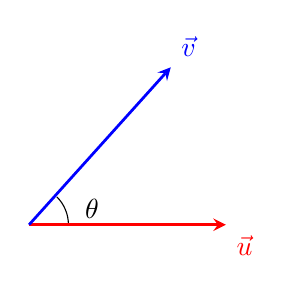
\begin{tikzpicture}
      \node[] at (0.8, 0.2)   (a) {$\theta$};
      \draw (0.5,0) arc (0:45:0.5) ;
      \draw[line width=1pt,-stealth,red](0,0)--(2.5,0)node[below right]{$\vec{u}$};
      \draw[line width=1pt,-stealth, blue](0,0)--(1.8,2)node[above right]{$\vec{v}$};
       \end{tikzpicture}
      \end{center}

   For now, we will consider $\vec{u}$ to be a unit vector, since we primarily care about the direction of $\vec{u}$ rather than its magnitude. 

   We can then ask ourselves the following question: Can we write $\vec{v}$ as the sum of two vectors, one in the direction of $\vec{u}$ and then one perpendicular to $\vec{u}$?

   Fundamentally, we are re-orienting space so that $\vec{u}$ becomes our new unit vector $\vec{i}$.

   In doing so, since vectors $\vec{v}$ will mostly not entirely lie in the same direction of $\vec{u}$, we need to find a second basis vector for the plane containing $\vec{u}$ and $\vec{v}$. 

   Taking a hint from our standard coordiante system, $\vec{i}$ and $\vec{j}$ are perpendicular to each other (that is, they form a right angle), and so we choose our second basis vector $\vec{u}_\perp$ to be oriented towards $\vec{v}$ but forming a right angle with $\vec{u}$, as in the following diagram.
     
    \begin{center}
     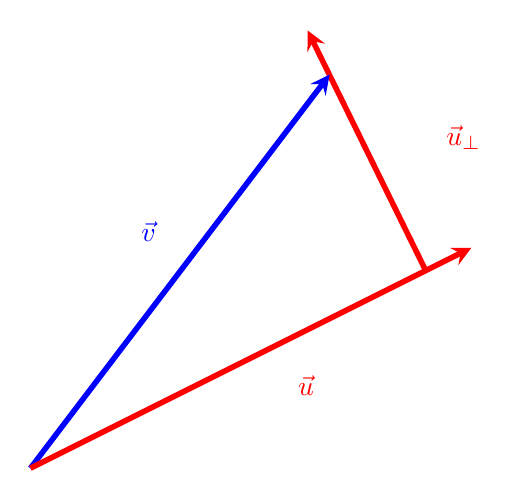
\begin{tikzpicture}
      \draw[line width=2pt,red,-stealth](3.02, .51)--(1.52,3.56);
      \node[red] at (3.5, 2.2)   (a) {$\vec{u}_{\perp}$};
     \node[red] at (1.5, -0.95)   (b) {$\vec{u}$};
      %\node[] at (5, 1)   (c) {$l$};
      \node[blue] at (-0.5, 1)   (d) {$\vec{v}$};
      % \draw [-,line width=1pt]  (-3,-2.5)--(5, 1.5);
    \draw[line width=2pt,blue,-stealth](-2, -2)--(1.8,3);
    \draw[line width=2pt,red,-stealth](-2, -2)--(3.6, 0.8);
    \end{tikzpicture}
     
    \end{center}

    The vectors in the diagram are drawn so that $\vec{v}$ is seen touching $\vec{u}_\perp$, rather than the usual coordiante system vectors joining at the origin. This is mostly to communicate that we can write $\vec{v}$ as a linear combination of $\vec{u}$ and $\vec{u}_\perp$, since $\vec{v}$ is in the plane now spanned by $\vec{u}$ and $\vec{u}_\perp$.

    The symbol ``$\perp$'' is notation for ``perpendicular'', meaning that the vectors form a right angle where they meet. 

    We now adopt the goal of writing $\vec{v}$ as the sum of two vectors, one in the direction of $\vec{u}$ and then another perpendicular to $\vec{u}$, such as in the following diagram. We'll denote the vector parallel to $\vec{u}$ as $\vec{v}_\parallel$, and the perpendicular vector $\vec{v}_\perp$, where $\parallel$ is ``parallel'', in reference to the vector $\vec{u}$.

    \begin{center}
      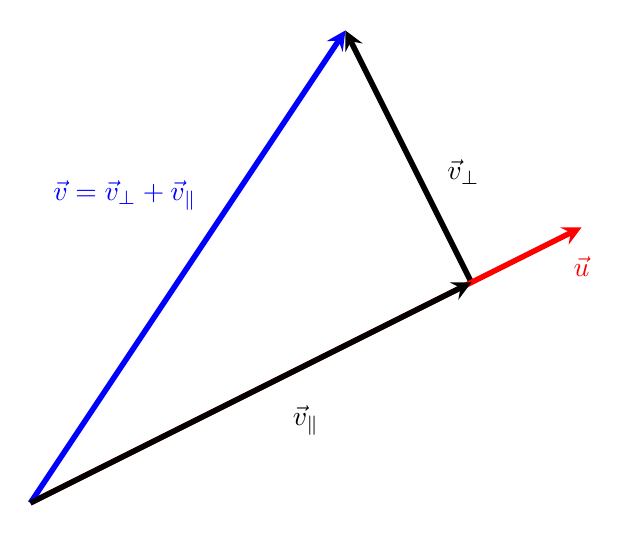
\begin{tikzpicture}
       \draw[line width=2pt,black,-stealth](3.6, 0.8)--(2,4);
       \node[black] at (3.5, 2.2)   (a) {$\vec{v}_{\perp}$};
      \node[black] at (1.5, -0.95)   (b) {$\vec{v}_{\parallel}$};
       \node[red] at (5, 1)   (c) {$\vec{u}$};
       \node[blue] at (-0.8, 1.9)   (d) {$\vec{v}=\vec{v}_{\perp}+\vec{v}_{\parallel}$};
       \draw[line width=2pt,red,-stealth]  (-2,-2)--(5, 1.5);
        %\draw [line width=1pt, red, stealth]  (-3,-2.5)--(5, 1.5);
     \draw[line width=2pt,blue,-stealth](-2, -2)--(2,4);
     \draw[line width=2pt,black,-stealth](-2, -2)--(3.6, 0.8);
     \end{tikzpicture}
      
     \end{center}

     To find the vectors $\vec{v}_\parallel$ and $\vec{v}_\perp$, we need to appeal to trigonometry and continue the motivation that we are re-orienting space so that $\vec{u}$ gives the new direction of the first basis vector. 

     With this appeal to trigonometry in mind, we note that assuming $\vec{v}_\perp$ and $\vec{v}_\parallel$ be perpendicular means that $\vec{v}_\perp, \vec{v}_\parallel,$ and $\vec{v}$ form the sides of a right triangle, and that the sides $\vec{v}_\parallel$ and $\vec{v}$ have the same angle measure $\theta$ as do $\vec{v}$ and $\vec{u}$.

     Because of this, as seen in the following diagram, we can find the lengths of the triangle sides using trigonometry.


     \begin{center}
      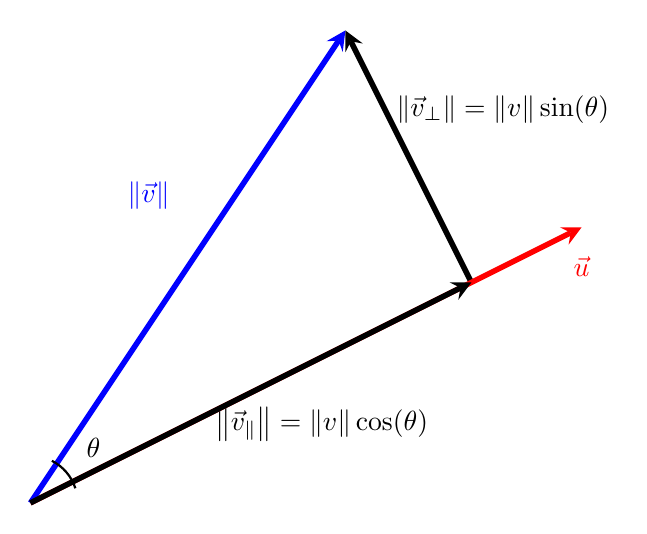
\begin{tikzpicture}
        % Axes
        %\draw[line width=0.5pt,gray!50] (-3, -3) -- (6, 1.5);
        %\draw[line width=0.5pt,gray!50] (-3, -3) -- (2, 5);
        
        % Vectors
        \draw[line width=2pt,black,-stealth](3.6, 0.8)--(2,4);
        \node[black] at (4, 3)   (a) {$\left\|\vec{v}_{\perp}\right\|=\left\|v\right\|\sin(\theta)$};
        \node[black] at (1.7, -1)   (b) {$\left\|\vec{v}_{\parallel}\right\|=\left\|v\right\|\cos(\theta)$};
        \node[red] at (5, 1)   (c) {$\vec{u}$};
        \node[blue] at (-0.5, 1.9)   (d) {$\norm{\vec{v}}$};
        \draw[line width=2pt,red,-stealth]  (-2,-2)--(5, 1.5);
        \draw[line width=2pt,blue,-stealth](-2, -2)--(2,4);
        \draw[line width=2pt,black,-stealth](-2, -2)--(3.6, 0.8);
        
        % Angle arc
        \draw[thick,-] (-2,-2) ++(18:0.6) arc[start angle=18, end angle=63, radius=0.6];
        \node[black] at (-1.2, -1.3) {$\theta$};

      \end{tikzpicture}
    \end{center}
     
     We are particularly interested in $\norm{\vec{v}_\parallel}$, since the vector $\vec{v}_\parallel$ is in $\mbox{span}(\vec{u})$, meaning it is within our desired first $1$-dimensional subspace. $\vec{v}_\parallel$ is called the \emph{projection} of $\vec{v}$ onto $\vec{u}$. 

     Moreover, we would rather not have to deal with trigonometric functions (this is, after all, \emph{linear} algebra), and so we seek a calculation for the length of $\norm{\vec{v}_\parallel}$ ideally in terms of $\vec{u}$ and $\vec{v}$, and more ideally the result of some linear calculation.
     
     This brings us to our first important linear transformation, the \emph{dot product}, which is the solution to our projection problem of finding the length of $\vec{v}_\parallel$ (and hence being able to explicitly write $\vec{v}_\parallel$ as $\norm{\vec{v}_\parallel}\vec{u}$ since $\vec{u}$ is a unit vector).

     \begin{definition}
      For a vector $\vec{u}=\begin{bmatrix}
         u_1\\\vdots \\ u_n
      \end{bmatrix}$ in $\RR^n$, the linear transformation defined by the $1\times n$ matrix $[u_1\ \ldots\ u_n]$ gives the \emph{dot product} of any vector $\vec{v}$ with $\vec{u}$. 
      
      The linear transformation is usually denoted $\vec{u}\cdot$, and the matrix multiplication $[u_1\ \ldots\ u_n]\begin{bmatrix}
      v_1 \\ \vdots \\v_n
      \end{bmatrix}$ is usually denoted $\vec{u}\cdot \vec{v}$, called ``$\vec{u}$ dot $\vec{v}$''.
     \end{definition}

     Here's a video introducing the dot product as the main idea of the chapter, and going over what much of what is worked out in the text below:

     %\begin{center}
      %\youtube{https://www.youtube.com/watch?v=LyGKycYT2v0}
     %\end{center}

     To understand why $\vec{u}\cdot\vec{v}$ gives us our desired projection, we need to work out the details of what is perhaps the most lengthy collection of abstract calculations in this book. There are thankfully few, and understanding $\vec{u}\cdot\vec{v}$ in terms of projections is very important, so we must suffer through!

     \begin{explanation}
      Let's re-state our goal. We know that $\norm{\vec{v}_\parallel}$, the projection of $\vec{v}$ onto the direction vector $\vec{u}$, is calculated as $\vec{v}\cos(\theta)$, and that ideally we would find some linear means of determining this length. 

      So, we dig deep and utilize some trigonometry, namely the Law of Cosines, and then utilize some algebra to solve for a more convenient representation of $\norm{\vec{v}_\parallel}$.

      First, consider a slightly different triangle, the triangle made by $\vec{v}$, $\vec{u}$, and $\vec{u}-\vec{v}$, seen here:

      \begin{center}
        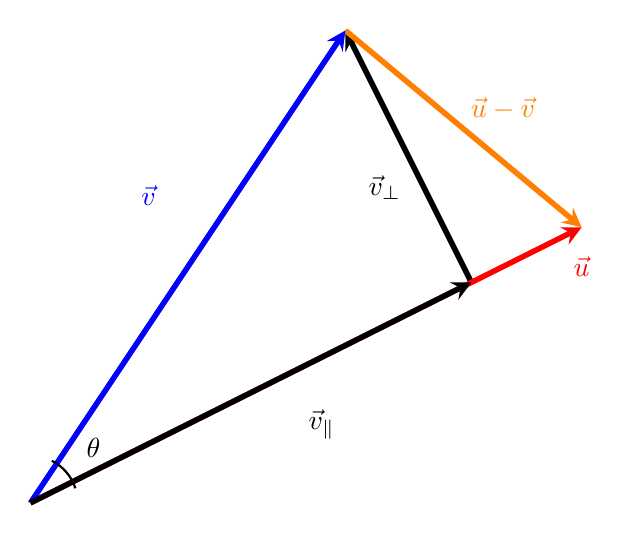
\begin{tikzpicture}
          % Axes
          %\draw[line width=0.5pt,gray!50] (-3, -3) -- (6, 1.5);
          %\draw[line width=0.5pt,gray!50] (-3, -3) -- (2, 5);
          
          % Vectors
          \draw[line width=2pt,black,-stealth](3.6, 0.8)--(2,4);
          \node[orange] at (4, 3)   (a) {$\vec{u}-\vec{v}$};
          \node[black] at (2.5,2) (e) {$\vec{v}_\perp$};
          \node[black] at (1.7, -1)   (b) {$\vec{v}_{\parallel}$};
          \node[red] at (5, 1)   (c) {$\vec{u}$};
          \node[blue] at (-0.5, 1.9)   (d) {$\vec{v}$};
          \draw[line width=2pt,red,-stealth]  (-2,-2)--(5, 1.5);
          \draw[line width=2pt,orange,-stealth] (2,4)--(5,1.5);
          \draw[line width=2pt,blue,-stealth](-2, -2)--(2,4);
          \draw[line width=2pt,black,-stealth](-2, -2)--(3.6, 0.8);
          
          % Angle arc
          \draw[thick,-] (-2,-2) ++(18:0.6) arc[start angle=18, end angle=63, radius=0.6];
          \node[black] at (-1.2, -1.3) {$\theta$};
  
        \end{tikzpicture}
      \end{center}
      
      The law of cosines tells us that the lengths of the larger triangle sides can be calculated (in relation to $\theta$) by the formula
      
      $$\norm{\vec{u}-\vec{v}}^2=\norm{\vec{u}}^2+\norm{\vec{v}}^2-2\norm{\vec{u}}\norm{\vec{v}}\cos(\theta).$$

      Luckily, this gives us exactly what we need to achieve our goals! Since $\left\|u\right\|=1$, $-2\norm{\vec{u}}\norm{\vec{v}}\cos(\theta)$ is very close to the length of our desired projection, $\norm{\vec{v}_\parallel}=\norm{\vec{v}}\cos(\theta)$. Moreover, we have a formula stated only in terms of our original vectors $\vec{u}$ and $\vec{v}$, as desired. 

      It gets even better, however, because for any vector $\vec{w}$, $\left\|\vec{w}\right\|^2=\sum_{k=1}^nw_k^2$, which gives us hope that we can find a linear calculation for our desired quantity (that is, sums and scalar multiplications).

      An old mathematical trick is to manipulate one side of an equation until it takes on a useful form, and then use that to your advantage to simplify some equation. we will do just that, working a little more closely with the calculation $\left\|\vec{u}-\vec{v}\right\|^2$.

      $$\left\|\vec{u}-\vec{v}\right\|^2=(u_1-v_1)^2+(u_2-v_2)^2+\ldots+(u_n-v_n)^2.$$

      This distributes to 

      $$(u_1^2-2u_1v_1+v_1^2)+(u_2^2-2u_2v_2+v_2^2)+\ldots+(u_n^2-2u_nv_n+v_n^2).$$

      We can rearrange the terms in the sum nicely to give us $\left\|\vec{u}\right\|^2$ and $\left\|\vec{v}\right|^2$, since the sum of the square components gives us the square norms of each vector!

      So grouping all of the $u_i^2$ and $v_i^2$ terms into their norm definitions gives us

      $$\left\|\vec{u}\right\|^2+\left\|\vec{v}\right|^2-2\left(u_1v_1+u_2v_2+\ldots+u_nv_n\right).$$

      Using summation notation to state the final product sum more concisely, and re-stating the original starting point of $\left|\vec{u}-\vec{v}\right\|^2$, we get

      $$\left\|\vec{u}-\vec{v}\right\|^2=\left\|\vec{u}\right\|^2+\left\|\vec{v}\right\|^2-2\sum_{k=1}^nu_kv_k.$$

      This, looks suspiciously similar to our statement of the Law of Cosines. In fact, we have two expressions equal to $\left\|\vec{u}-\vec{v}\right\|^2$, so we set those expressions equal to each other to get

      $$\norm{\vec{u}}^2+\norm{\vec{v}}^2-2\norm{\vec{u}}\norm{\vec{v}}\cos(\theta)=\left\|\vec{u}\right\|^2+\left\|\vec{v}\right\|^2-2\sum_{k=1}^nu_kv_k.$$

      Both sides of the equality have $\norm{\vec{u}}^2+\norm{\vec{v}}^2$, so those terms can cancel for simplification. Moreover, we can then divide both sides by $-2$ as well, to get the final result

      $$\norm{\vec{u}}\norm{\vec{v}}\cos(\theta)=\sum_{k=1}^nu_kv_k.$$

      We've done it! Since $\left\|u\right\|=1$, we've found the desired length of our projection $\norm{\vec{v}_\parallel}=\sum_{k=1}^nu_kv_k$. Even more exciting, $\sum_{k=1}^nu_kv_k$ is the sum of products, which hopefully screams at you the all-important phrase {\bf linear combination}!!!

      So, why the definition of the dot product as multiplication by the matrix $[u_1\ u_2\ \ldots\ u_n]$? Well, what is matrix multiplication but a linear combination? In fact, it's the same linear combination as our sum!

      Note that by definition of matrix multiplication, $[u_1\ u_2\ \ldots\ u_n]\begin{bmatrix}
        v_1\\v_2\\\vdots\\v_n
      \end{bmatrix}$ is the linear combination of the columns of $[u_1\ u_2\ \ldots\ u_n]$ with the coordinates of $\begin{bmatrix}
        v_1\\v_2\\\vdots\\v_n
      \end{bmatrix}$, which is exactly the sum $\sum_{k=1}^nu_kv_k$.

     \end{explanation}

    Stated more generally, let's write the \emph{dot product} in three equivalent ways:

    \begin{theorem}
      Let $\vec{u}$ and $\vec{v}$ be vectors in $\RR^n$. Then the dot product, denoted $\vec{u}\cdot\vec{v}$, is given as any of the following calculations:

      \begin{enumerate}
        \item The matrix product $[u_1\ u_2\ \ldots\ u_n]\begin{bmatrix}
        v_1\\v_2\\\vdots\\v_n
      \end{bmatrix}$
        \item The matrix product $[v_1\ v_2\ \ldots\ v_n]\begin{bmatrix}
        u_1\\u_2\\\vdots\\u_n
      \end{bmatrix}$
        \item The linear combination $\sum_{k=1}^nu_kv_k$.
        \item The product $\left\|u\right\|\left\|v\right\|\cos(\theta)$.
      \end{enumerate}
    \end{theorem}

    Each of these go beyond our original orthogonal projection case, where $\left\|u\right\|$ might not be a unit vector. 

    \begin{remark}
      We get a few nice results from the dot product. 

      First, note that this gives us a way to find the smallest angle between two vectors, as we can solve for $\cos(\theta)$ to get 

      $$\cos(\theta)=\frac{\vec{u}\cdot\vec{v}}{\left\|\vec{u}\right\|\left\|\vec{v}\right\|}.$$

      This is sometimes called the \emph{cosine similarity}, which is a very important calculation that underlies many machine learning models, such as large language models like ChatGPT.

      Also, the perpendicular projection $\vec{v}_\parallel$ is not quite able to be determined by a linear transformation, since $\vec{v}$ and $\vec{u}$ might not be unit vectors and hence there is a need to account for the product of their magnitudes. 

      We thus get the following definition of the \emph{orthogonal} projection of $\vec{v}$ onto $\vec{u}$.
    \end{remark}

    \begin{definition}
      If we \emph{orthogonally} project $\vec{v}$ onto $\vec{u}$, we denote the projection vector $\mbox{proj}(\vec{v})_{\vec{u}}$ (e.g. $\vec{v}$ is ``projected'' onto $\vec{u}$).
  
      
      The projection vector has length $\frac{\vec{u}\cdot\vec{v}}{\norm{\vec{u}}}$, and the projection vector itself is explicitly stated ask

      $$\mbox{proj}(\vec{v})_{\vec{u}}=\frac{\vec{u}\cdot\vec{v}}{\norm{\vec{u}}}\frac{\vec{u}}{\norm{\vec{u}}}.$$


      Note that this aligns with our original projection length of $\left\|\vec{v}\right\|\cos(\theta)$, and that for simplicity the divisions by $\norm{\vec{u}}$ are often combined in the formula for the projection vector into a square denominator.
    \end{definition}

    The term ``orthogonal'' will have more significance in the next section, but for now it is analogous to ``perpendicular''.
     
\end{document}